\begin{figure}[h]
	\centering
	\captionsetup{justification=centering}
	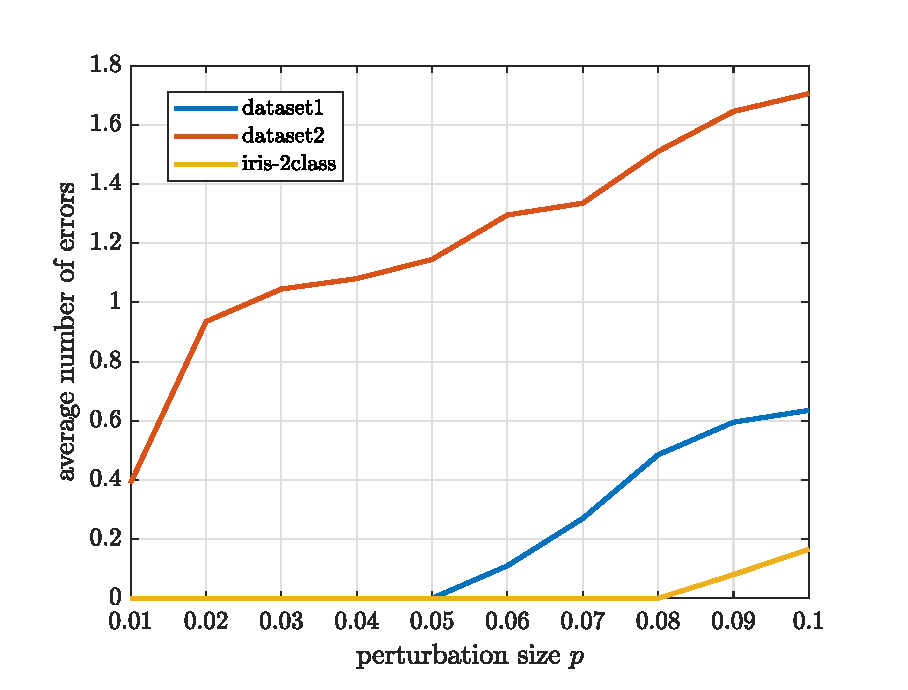
\includegraphics[width=.45\textwidth]{averages}
	\caption{Error average vs perturbation size.}
	\label{averages}
\end{figure}

Prediction errors differ from each datasets since they all have a different spread of data. We'll start off by comparing the first two which are fairly similar between each other. Looking at the average number of errors in figure \ref{averages} we can immediately distinguish that the second dataset if far more prone to errors even with small perturbations. The way data is spread in such dataset makes it hard to find a hyperplane that accurately divides both classes, in other words, a great number of observations are lying closer to the decision boundary making them possible candidates for misclassification.

As for the modified iris dataset, even though the number of observations is  greater than in the previous two, the average number of errors is considerably low. The particular spread of the data makes it easier to split the two classes and there are a vast amount of hyperplanes that could accurately classify both classes.
